\section{Consuntivo di periodo e preventivo a finire}
In questa sezione verranno indicate le spese, totali e per ruolo, sostenute al termine di ciascuna fase.
Il bilancio presentato potrà essere:
\begin{itemize}
	\item \textbf{positivo:} se il totale preventivato è superiore ai valori del consuntivo;
	\item \textbf{pari:} se il totale preventivato è pari ai valori del consuntivo;
	\item \textbf{negativo:} se il totale preventivato è inferiore ai valori del consuntivo.
\end{itemize}
Verrà inoltre presentato un preventivo a finire che terrà conto dei soli periodi rendicontati.

\subsection{Periodo di Analisi}
\subsubsection{Consuntivo di periodo}
\rowcolors{2}{lightRowColor}{darkRowColor}
\begin{longtable}{
		>{\centering}p{0.25\textwidth}
		>{\centering}p{0.08\textwidth}
		>{\centering}p{0.08\textwidth}
		>{\centering}p{0.15\textwidth}
		>{\centering\arraybackslash}p{0.15\textwidth} }
	
	\coloredTableHead
	\textbf{\color{white}Ruolo} &
	\textbf{\color{white}Ore} &
	\textbf{\color{white}Delta ore} &
	\textbf{\color{white}Costo in \euro{}} &
	\textbf{\color{white}Delta costo}
	\tabularnewline
	\endhead
	
	% Contenuto della tabella
	% Ruolo & OreEffettive & DeltaOre & Costo & DeltaCosto \\
	Responsabile    & 28 & -2 &   840,00 & -60 \\
	Amministratore  & 70 & +0 & 1.400,00 & +0,00 \\
	Analista        & 63 & +3 & 1.575,00 & +75,00 \\
	Progettista     & 20 & +0 &   440,00 & +0,00 \\
	Programmatore   & -  & -  & -        & - \\
	Verificatore    & 74 & +4 & 1.110,00 & +60,00 \\
	\textbf{Totale Effettivo} & \multicolumn{2}{c}{\textbf{255}} & \multicolumn{2}{c}{\textbf{5365,00}} \\
	\textbf{Delta} & \multicolumn{2}{c}{\textbf{+4}} & \multicolumn{2}{c}{\textbf{+75,00}} \\
	
	\rowcolor{white}\caption{Consuntivo per il periodo di Analisi}	\\
	
\end{longtable}

\subsubsection{Conclusione}
Come riportato nella tabella del consuntivo per il periodo di Analisi, il preventivo orario per i ruoli di Amministratore e Progettista si è rivelato sufficiente per svolgere il lavoro previsto; si è rivelato  invece necessario dedicare più ore lavorative rispetto a quanto preventivato per i ruoli di Analista e Verificatore, mentre è stato impiegato un monte ore ridotto per il ruolo di Responsabile di Progetto. Di seguito sono riportate le motivazioni:
\begin{itemize}
	\item \textbf{Responsabile di Progetto:} sono state impiegate meno ore rispetto a quelle previste data la minore difficoltà di stesura del \textit{\PdP{} 1.0.0} e di pianificazione del lavoro rispetto a quanto previsto;
	\item \textbf{Analista:} alcuni requisiti hanno presentato delle difficoltà di comprensione, con un conseguente aumento del monte ore necessario per la loro comprensione e stesura all'interno dell'\textit{\AdR{} 1.0.0};
	\item \textbf{Verificatore:} l'aggiornamento delle \textit{\NdP{} 1.0.0} e l'applicazione scorretta di alcune norme causata dall'inesperienza dei membri del gruppo ha portato ad un aumento delle ore spese per questo ruolo.
\end{itemize}

\subsubsection{Preventivo a finire}
Il bilancio finale è negativo. Nonostante ciò, non riteniamo necessario attuare misure di mitigazione o modifiche alla pianificazione dei periodi successivi, in quanto, oltre al fatto che il periodo di Analisi non è rendicontato, siamo riusciti ad individuare le situazioni e le motivazioni che hanno portato a richiedere ore di lavoro aggiuntive rispetto a quelle preventivate. Ciascun componente del gruppo si impegnerà per cercare di evitare che situazioni di questo tipo si possano ripetere nei periodi successivi.


\subsection{Periodo di Consolidamento dei Requisiti}
\subsubsection{Consuntivo di periodo}
\rowcolors{2}{lightRowColor}{darkRowColor}
\begin{longtable}{
		>{\centering}p{0.25\textwidth}
		>{\centering}p{0.08\textwidth}
		>{\centering}p{0.08\textwidth}
		>{\centering}p{0.15\textwidth}
		>{\centering\arraybackslash}p{0.15\textwidth} }
	
	\coloredTableHead
	\textbf{\color{white}Ruolo} &
	\textbf{\color{white}Ore} &
	\textbf{\color{white}Delta ore} &
	\textbf{\color{white}Costo in \euro{}} &
	\textbf{\color{white}Delta costo}
	\tabularnewline
	\endhead
	
	% Contenuto della tabella
	% Ruolo & OreEffettive & DeltaOre & Costo & DeltaCosto \\
	Responsabile    & 5  & +0 & 150,00 & +0,00 \\
	Amministratore  & 6  & +0 & 120,00 & +0,00 \\
	Analista        & 10 & +0 & 250,00 & +0,00 \\
	Progettista     & -  & -  & -       & +0,00 \\
	Programmatore   & -  & -  & -       & +0,00 \\
	Verificatore    & 15 & +0 & 225,00 & +0,00 \\
	\textbf{Totale Effettivo} & \multicolumn{2}{c}{\textbf{36}} & \multicolumn{2}{c}{\textbf{745,00}} \\
	\textbf{Delta} & \multicolumn{2}{c}{\textbf{+0}} & \multicolumn{2}{c}{\textbf{+0,00}} \\
	
	\rowcolor{white}\caption{Consuntivo per il periodo di Consolidamento dei Requisiti}	\\
	
\end{longtable}

\subsubsection{Conclusione}
Il totale delle ore preventivate per il periodo di Consolidamento dei Requisiti si è rivelato corretto per svolgere il lavoro pianificato.
\subsubsection{Preventivo a finire}
Il bilancio finale è pari. Non si rendono quindi necessarie misure di mitigazione o modifiche alla pianificazione dei periodi successivi.

\subsection{Periodo di Progettazione Architetturale}
\subsubsection{Consuntivo di periodo}
\rowcolors{2}{lightRowColor}{darkRowColor}
\begin{longtable}{
		>{\centering}p{0.25\textwidth}
		>{\centering}p{0.08\textwidth}
		>{\centering}p{0.08\textwidth}
		>{\centering}p{0.15\textwidth}
		>{\centering\arraybackslash}p{0.15\textwidth} }
	
	\coloredTableHead
	\textbf{\color{white}Ruolo} &
	\textbf{\color{white}Ore} &
	\textbf{\color{white}Delta ore} &
	\textbf{\color{white}Costo in \euro{}} &
	\textbf{\color{white}Delta costo}
	\tabularnewline
	\endhead
	
	% Contenuto della tabella
	% Ruolo & OreEffettive & DeltaOre & Costo & DeltaCosto \\
	Responsabile    & 12 & +0 &   360,00 & +  0,00 \\
	Amministratore  & 24 & +0 &   480,00 & +  0,00 \\
	Analista        & 35 & +2 &   875,00 & + 50,00 \\
	Progettista     & 67 & -5 & 1.474,00 & -110,00 \\
	Programmatore   & 35 & -4 &   525,00 & - 60,00 \\
	Verificatore    & 68 & +0 & 1.020,00 & +  0,00 \\
	\textbf{Totale Effettivo} & \multicolumn{2}{c}{\textbf{241}} & \multicolumn{2}{c}{\textbf{4.734,00}} \\
	\textbf{Delta} & \multicolumn{2}{c}{\textbf{-7}} & \multicolumn{2}{c}{\textbf{-120,00}} \\
	
	\rowcolor{white}\caption{Consuntivo per il periodo di Progettazione Architetturale}	\\
	
\end{longtable}

\subsubsection{Conclusione}
Come riportato nella tabella del consuntivo per il periodo di Progettazione Architetturale, il preventivo orario per i ruoli di Responsabile, Amministratore e Verificatore si è rivelato sufficiente per svolgere il lavoro pianificato. \\
Si è rivelato necessario dedicare più ore lavorative rispetto a quanto preventivato per il ruolo di Analista, mentre è stato impiegato un monte ore ridotto per i ruoli di Progettista e Programmatore. Di seguito sono riportate le motivazioni:
\begin{itemize}
	\item \textbf{Analista:} la comprensione delle indicazioni ricevute nell'esito della \textit{Revisione dei Requisiti} e la conseguente correzione del documento dell'\textit{AdR{} 2.0.0}, hanno richiesto alcune ore di lavoro in più rispetto a quelle preventivate;
	\item \textbf{Progettista:} le molte ore di studio individuale impiegate nel periodo di Consolidamento dei Requisiti riguardo le tecnologie ritenute potenzialmente utili per lo sviluppo del prodotto\ped{\textit{G}}, hanno permesso di poter impiegare meno ore di quanto pianificato per l'individuazione delle tecnologie e delle librerie adatte allo sviluppo del prodotto\ped{\textit{G}};
	\item \textbf{Programmatore:} grazie alle ore di studio individuali descritte nel punto precedente e all'adeguata scelta delle tecnologie e delle librerie, la codifica del \textit{Proof of Concept} ha richiesto meno ore di lavoro rispetto a quelle preventivate.
\end{itemize}

\subsubsection{Preventivo a finire}
Il bilancio finale è positivo. Ciò è dovuto soprattutto alla scelta iniziale delle tecnologie e delle librerie da utilizzare, che si è rivelata adeguata e ci ha permesso di risparmiare delle ore di lavoro nelle attività di progettazione e di codifica del \textit{Proof of Concept} rispetto a quanto avevamo preventivato. \\
Intendiamo utilizzare l'ammontare risparmiato in questo periodo per assegnare alcune ore supplementari al ruolo dell'Analista nel periodo di Progettazione di Dettaglio e Codifica, in quanto potrebbe essere necessario apportare modifiche al documento dell'\textit{AdR{} 2.0.0}, seguendo eventuali indicazioni ricevute a seguito dell'esito della \textit{Revisione di Progettazione}.

\subsection{Periodo di Progettazione di Dettaglio e Codifica}
Vengono riportati di seguito i consuntivi degli 8 incrementi che costituiscono il periodo considerato.

\subsubsection{9$^{\circ}$ Incremento}
		\subsubsubsection{Prospetto orario}
		Durante il 9$^{\circ}$ Incremento la distribuzione oraria preventivata dei ruoli di ogni componente del gruppo sarà la seguente:
		\rowcolors{2}{lightRowColor}{darkRowColor}
		\begin{longtable}{
				>{\centering}p{0.25\textwidth}
				>{\centering}p{0.05\textwidth}
				>{\centering}p{0.05\textwidth}
				>{\centering}p{0.05\textwidth}
				>{\centering}p{0.05\textwidth}
				>{\centering}p{0.05\textwidth}
				>{\centering}p{0.05\textwidth}
				>{\centering\arraybackslash}p{0.15\textwidth} }
			
			\coloredTableHead
			\textbf{\color{white}Nome} &
			\textbf{\color{white}Rp} &
			\textbf{\color{white}As} &
			\textbf{\color{white}An} &
			\textbf{\color{white}Pt} &
			\textbf{\color{white}Pr} &
			\textbf{\color{white}Vf} &
			\textbf{\color{white}Totale}
			\tabularnewline
			\endhead
			
			% Contenuto della tabella
			%    Rp & As & An & Pt & Pr & Vf & Totale \\
			\VB & - & 2  & - & - & - & 4 & 6 \\
			\LB & - & -  & - & 4 & - & - & 4 \\
			\NF & - & 4  & - & - & - & - & 4 \\
			\EG & 2 & -  & - & 2 & - & - & 4 \\
			\FJ & - & -  & - & - & - & 4 & 4 \\
			\MP & - & -  & - & 2 & - & 3 & 5 \\
			\AS & - & -  & - & 2 & - & 2 & 4 \\
			\AZ & - & 2  & - & - & - & 2 & 4 \\
			\textbf{Ore totali per ruolo} & 2 & 8 & 0 & 10 & 0 & 15 & 35 \\
			
			\rowcolor{white}\caption {Suddivisione oraria del 9$^{\circ}$ Incremento} \\
			
		\end{longtable}
		
		% Grafico
		\begin{figure}[H]
			\centering
			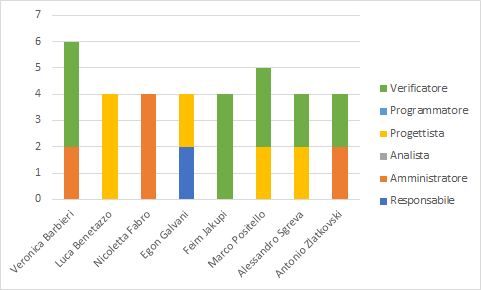
\includegraphics[width=0.7\textwidth]{./res/img/preventivi/inc9_po.png}
			\caption{Suddivisione oraria del 9$^{\circ}$ Incremento}
		\end{figure}
	
		\subsubsubsection{Prospetto economico}
		In base al prospetto orario, quello economico sarà il seguente: 
		\rowcolors{2}{lightRowColor}{darkRowColor}
		\begin{longtable}{
				>{\centering}p{0.25\textwidth}
				>{\centering}p{0.05\textwidth}
				>{\centering\arraybackslash}p{0.15\textwidth} }
			
			\coloredTableHead
			\textbf{\color{white}Ruolo} &
			\textbf{\color{white}Ore} &
			\textbf{\color{white}Costo in \euro{}}
			\tabularnewline
			\endhead
			
			% Contenuto della tabella
			% Ruolo & Ore & Costo \\
			Responsabile    & 2  & 60,00 \\
			Amministratore  & 8  & 160,00 \\
			Analista        & 0  & 0,00 \\
			Progettista     & 10  & 220,00 \\
			Programmatore   & 0  & 0,00 \\
			Verificatore    & 15  & 225,00 \\
			\textbf{Totale} & 35 & 665,00 \\
			
			\rowcolor{white}\caption {Prospetto dei costi per il 9$^{\circ}$ Incremento}	\\
			
		\end{longtable}
		
		% Grafico
		Rappresentazione grafica della distribuzione dei ruoli:
		\begin{figure}[H]
			\centering
			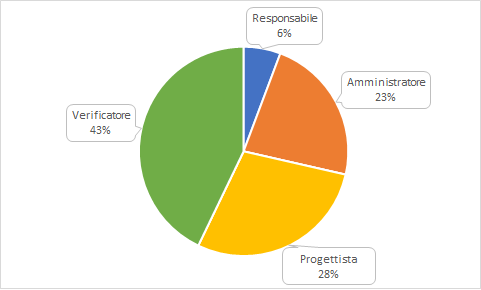
\includegraphics[width=0.7\textwidth]{./res/img/preventivi/inc9_pe.png}
			\caption{Prospetto economico del 9$^{\circ}$ Incremento}
		\end{figure}
\subsubsection{10$^{\circ}$ Incremento}
	
	\subsubsubsection{Consuntivo}
					
		\begin{longtable}{
				>{\centering}p{0.25\textwidth}
				>{\centering}p{0.08\textwidth}
				>{\centering}p{0.08\textwidth}
				>{\centering}p{0.15\textwidth}
				>{\centering\arraybackslash}p{0.15\textwidth} }
			
			\coloredTableHead
			\textbf{\color{white}Ruolo} &
			\textbf{\color{white}Ore} &
			\textbf{\color{white}Delta ore} &
			\textbf{\color{white}Costo in \euro{}} &
			\textbf{\color{white}Delta costo}
			\tabularnewline
			\endhead
			
			% Contenuto della tabella
			% Ruolo & OreEffettive & DeltaOre & Costo & DeltaCosto \\
			Responsabile    & 4 & +0 &   120,00 & +  0,00 \\
			Amministratore  & 4 & +0 &   80,00 & +  0,00 \\
			Analista        & 0 & +0 &   0,00 & + 0,00 \\
			Progettista     & 39 & +4 & 858,00 & + 88,00 \\
			Programmatore   & 23 & -2 &  345,00 & - 30,00 \\
			Verificatore    & 25 & +0 & 375,00 & + 0,00 \\
			\textbf{Totale Effettivo} & \multicolumn{2}{c}{\textbf{95}} & \multicolumn{2}{c}{\textbf{1778,00}} \\
			\textbf{Delta} & \multicolumn{2}{c}{\textbf{+2}} & \multicolumn{2}{c}{\textbf{+58,00}} \\
			
			\rowcolor{white}\caption{Consuntivo per il 10$^{\circ}$ Incremento}	\\
			
		\end{longtable}
		
	\subsubsubsection{Conclusioni}
	In questo periodo il gruppo si è impegnato nella progettazione e scelta dell'architettura da applicare al prodotto\ped{\textit{G}}. Tale procedimento ha richiesto più tempo del previsto, portando alla necessità di un numero di ore superiore a quanto pianificato per il ruolo di Progettista. \\
	L'attività di codifica è stata leggermente meno dispendiosa del previsto, a causa dell'utilizzo del prototipo ottenuto dalla fase precedente. 
	
	\subsubsubsection{Preventivo a finire rispetto al periodo}
	Il bilancio è \textbf{negativo}, con una spesa in eccesso di \textbf{58,00\euro{}}. Non si ritiene necessaria alcuna ripianificazione, poichè la somma non è significativa. 
	Il soddisfacimento degli obiettivi pianificati ha richiesto un quantitativo di ore superiore a quanto previsto, che hanno portato a questo bilancio negativo.
	
	\subsubsubsection{Preventivo a finire complessivo}	
	Date le considerazioni precedenti su costi e obiettivi, il preventivo complessivo resta invariato.
\subsubsection{11$^{\circ}$ Incremento}
	
	\subsubsubsection{Consuntivo}
		\begin{longtable}{
				>{\centering}p{0.25\textwidth}
				>{\centering}p{0.08\textwidth}
				>{\centering}p{0.08\textwidth}
				>{\centering}p{0.15\textwidth}
				>{\centering\arraybackslash}p{0.15\textwidth} }
			
			\coloredTableHead
			\textbf{\color{white}Ruolo} &
			\textbf{\color{white}Ore} &
			\textbf{\color{white}Delta ore} &
			\textbf{\color{white}Costo in \euro{}} &
			\textbf{\color{white}Delta costo}
			\tabularnewline
			\endhead
			
			% Contenuto della tabella
			% Ruolo & OreEffettive & DeltaOre & Costo & DeltaCosto \\
			Responsabile    & 3 & +0 &   90,00 & +  0,00 \\
			Amministratore  & 4 & +0 &   80,00 & +  0,00 \\
			Analista        & 0 & +0 &   0,00 & + 0,00 \\
			Progettista     & 10 & +0 & 220,00 & + 0,00 \\
			Programmatore   & 35 & -7 &   525,00 &  -105,00 \\
			Verificatore    & 15 & +0 & 225,00 & + 0,00 \\
			\textbf{Totale Effettivo} & \multicolumn{2}{c}{\textbf{64}} & \multicolumn{2}{c}{\textbf{1140,00}} \\
			\textbf{Delta} & \multicolumn{2}{c}{\textbf{-10}} & \multicolumn{2}{c}{\textbf{-105,00}} \\
			
			\rowcolor{white}\caption{Consuntivo per l'11$^{\circ}$ Incremento}	\\
			
		\end{longtable}
		
	\subsubsubsection{Conclusioni}
	In questo periodo il gruppo si è impegnato principalmente nell'adattare la struttura del prototipo ottenuto dalla fase precedente alla progettazione identificata nell'Incremento 10. Tale attività ha richiesto un notevole numero di ore di codifica in meno rispetto a quanto previsto, poichè la struttura del prototipo seguiva già in parte quella decisa durante la progettazione. 
	
	\subsubsubsection{Preventivo a finire rispetto al periodo}
	Il bilancio è \textbf{positivo}, con un risparmio di \textbf{105,00\euro{}}.  Tale somma
	andrà a bilanciare il leggero deficit ottenuto nell'Incremento precedente. La differenza
	rispetto ai costi preventivati fino a questo punto sarà quindi poco consistente, perciò non si
	reputa necessaria una ripianificazione delle attività di progetto.
	
	\subsubsubsection{Preventivo a finire complessivo}	
	Date le considerazioni precedenti, il preventivo complessivo resta invariato.
\subsubsection{12$^{\circ}$ Incremento}
		\subsubsubsection{Prospetto orario}
		Durante il 12$^{\circ}$ incremento la distribuzione oraria preventivata dei ruoli di ogni componente del gruppo sarà la seguente:
		\rowcolors{2}{lightRowColor}{darkRowColor}
		\begin{longtable}{
				>{\centering}p{0.25\textwidth}
				>{\centering}p{0.05\textwidth}
				>{\centering}p{0.05\textwidth}
				>{\centering}p{0.05\textwidth}
				>{\centering}p{0.05\textwidth}
				>{\centering}p{0.05\textwidth}
				>{\centering}p{0.05\textwidth}
				>{\centering\arraybackslash}p{0.15\textwidth} }
			
			\coloredTableHead
			\textbf{\color{white}Nome} &
			\textbf{\color{white}Rp} &
			\textbf{\color{white}As} &
			\textbf{\color{white}An} &
			\textbf{\color{white}Pt} &
			\textbf{\color{white}Pr} &
			\textbf{\color{white}Vf} &
			\textbf{\color{white}Totale}
			\tabularnewline
			\endhead
			
			% Contenuto della tabella
			%    Rp & As & An & Pt & Pr & Vf & Totale \\
			\VB & - & -  & - & - & 10 & - & 10 \\
			\LB & - & -  & - & 4 & 10 & - & 14 \\
			\NF & - & -  & - & - & 10 & - & 10 \\
			\EG & - & -  & - & - & 10 & 2 & 12 \\
			\FJ & 2 & -  & - & 4 & - & 1 & 7 \\
			\MP & 1 & -  & - & - & 5 & 2 & 8 \\
			\AS & - & -  & - & 2 & - & 5 & 7 \\
			\AZ & - & 3  & - & - & - & 5 & 8 \\
			\textbf{Ore totali per ruolo} & 3 & 3 & 0 & 10 & 45 & 15 & 76 \\
			
			\rowcolor{white}\caption {Suddivisione oraria del 12$^{\circ}$ incremento} \\
			
		\end{longtable}
		
		% Grafico
		\begin{figure}[H]
			\centering
			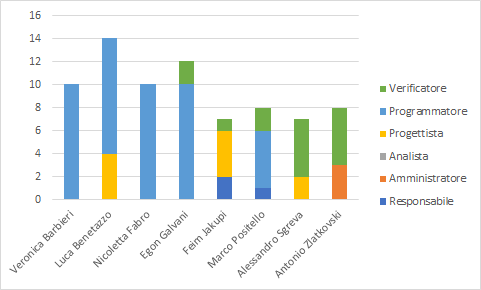
\includegraphics[width=0.7\textwidth]{./res/img/preventivi/inc12_po.png}
			\caption{Suddivisione oraria del 12$^{\circ}$ incremento}
		\end{figure}
	
		\subsubsubsection{Prospetto economico}
		In base al prospetto orario, quello economico sarà il seguente: 
		\rowcolors{2}{lightRowColor}{darkRowColor}
		\begin{longtable}{
				>{\centering}p{0.25\textwidth}
				>{\centering}p{0.05\textwidth}
				>{\centering\arraybackslash}p{0.15\textwidth} }
			
			\coloredTableHead
			\textbf{\color{white}Ruolo} &
			\textbf{\color{white}Ore} &
			\textbf{\color{white}Costo in \euro{}}
			\tabularnewline
			\endhead
			
			% Contenuto della tabella
			% Ruolo & Ore & Costo \\
			Responsabile    & 3  & 90,00 \\
			Amministratore  & 3  & 60,00 \\
			Analista        & 0  & 0,00 \\
			Progettista     & 10  & 220,00 \\
			Programmatore   & 45 & 675,00 \\
			Verificatore    & 15  & 225,00 \\
			\textbf{Totale} & 76 & 1270,00 \\
			
			\rowcolor{white}\caption {Prospetto dei costi per il 12$^{\circ}$ incremento}	\\
			
		\end{longtable}
		
		% Grafico
		Rappresentazione grafica della distribuzione dei ruoli:
		\begin{figure}[H]
			\centering
			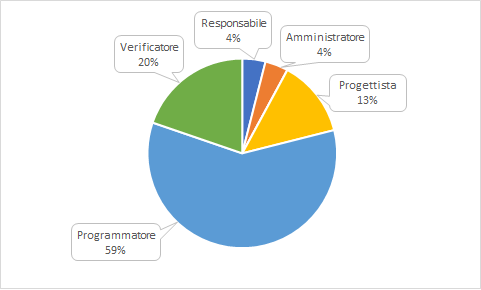
\includegraphics[width=0.7\textwidth]{./res/img/preventivi/inc12_pe.png}
			\caption{Prospetto economico del 12$^{\circ}$ incremento}
		\end{figure}
\subsubsection{13$^{\circ}$ Incremento}
	
	\subsubsubsection{Consuntivo}
		\begin{longtable}{
				>{\centering}p{0.25\textwidth}
				>{\centering}p{0.08\textwidth}
				>{\centering}p{0.08\textwidth}
				>{\centering}p{0.15\textwidth}
				>{\centering\arraybackslash}p{0.15\textwidth} }
			
			\coloredTableHead
			\textbf{\color{white}Ruolo} &
			\textbf{\color{white}Ore} &
			\textbf{\color{white}Delta ore} &
			\textbf{\color{white}Costo in \euro{}} &
			\textbf{\color{white}Delta costo}
			\tabularnewline
			\endhead
			
			% Contenuto della tabella
			% Ruolo & OreEffettive & DeltaOre & Costo & DeltaCosto \\
			Responsabile    & 3 & +0 &   90,00 & +  0,00 \\
			Amministratore  & 3 & +0 &   60,00 & +  0,00 \\
			Analista        & 0 & +0 &   0,00 & + 0,00 \\
			Progettista     & 10 & +0 & 220,00 & + 0,00 \\
			Programmatore   & 27 & -3 &   405,00 &  -45,00 \\
			Verificatore    & 12 & +0 & 180,00 & + 0,00 \\
			\textbf{Totale Effettivo} & \multicolumn{2}{c}{\textbf{55}} & \multicolumn{2}{c}{\textbf{955,00}} \\
			\textbf{Delta} & \multicolumn{2}{c}{\textbf{-3}} & \multicolumn{2}{c}{\textbf{-45,00}} \\
			
			\rowcolor{white}\caption{Consuntivo per il 13$^{\circ}$ Incremento}	\\
			
		\end{longtable}
		
	
	\subsubsubsection{Conclusioni}
	In questo periodo il gruppo si è impegnato principalmente nell'implementare la funzionalità di eliminazione di una funzione dalla piattaforma \textit{Etherless}. L'attività di codifica ha richiesto un numero di ore inferiore a quanto preventivato, in quanto tale funzionalità segue un pattern di comunicazione tra i moduli\ped{\textit{G}} molto simile a quello richiesto da altre funzionalità già implementate. 
	
	\subsubsubsection{Preventivo a finire rispetto al periodo}
	Il bilancio è \textbf{positivo}, con un risparmio di \textbf{45,00\euro{}}. Non si ritiene necessaria alcuna ripianificazione, poichè la somma non è significativa. 
	Gli obiettivi pianificati sono stati raggiunti nei tempi stabiliti, consentendo l'avanzamento delle attività senza ritardi.
	
	\subsubsubsection{Preventivo a finire complessivo}	
	Date le considerazioni precedenti, il preventivo complessivo resta invariato.
\subsubsection{14$^{\circ}$ Incremento}
		\subsubsubsection{Prospetto orario}
		Durante il quattordicesimo incremento la distribuzione oraria preventivata dei ruoli di ogni componente del gruppo sarà la seguente:
		\rowcolors{2}{lightRowColor}{darkRowColor}
		\begin{longtable}{
				>{\centering}p{0.25\textwidth}
				>{\centering}p{0.05\textwidth}
				>{\centering}p{0.05\textwidth}
				>{\centering}p{0.05\textwidth}
				>{\centering}p{0.05\textwidth}
				>{\centering}p{0.05\textwidth}
				>{\centering}p{0.05\textwidth}
				>{\centering\arraybackslash}p{0.15\textwidth} }
			
			\coloredTableHead
			\textbf{\color{white}Nome} &
			\textbf{\color{white}Rp} &
			\textbf{\color{white}As} &
			\textbf{\color{white}An} &
			\textbf{\color{white}Pt} &
			\textbf{\color{white}Pr} &
			\textbf{\color{white}Vf} &
			\textbf{\color{white}Totale}
			\tabularnewline
			\endhead
			
			% Contenuto della tabella
			%    Rp & As & An & Pt & Pr & Vf & Totale \\
			\VB & 3 & -  & - & 3 & - & - & 6 \\
			\LB & - & -  & - & 3 & - & - & 3 \\
			\NF & - & -  & - & 2 & 1 & - & 3 \\
			\EG & - & -  & - & - & 2 & 6 & 8 \\
			\FJ & - & 1  & - & - & 3 & - & 4 \\
			\MP & - & 3  & - & - & 2 & - & 5 \\
			\AS & - & -  & - & - & 3 & 4 & 7 \\
			\AZ & - & -  & - & - & 5 & - & 5 \\
			\textbf{Ore totali per ruolo} & 3 & 4 & 0 & 8 & 16 & 10 & 41 \\
			
			\rowcolor{white}\caption {Suddivisione oraria del quattordicesimo incremento} \\
			
		\end{longtable}
		
		% Grafico
		\begin{figure}[h]
			\centering
			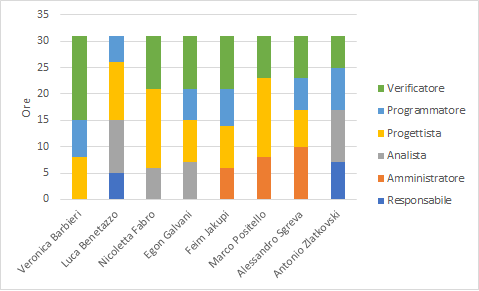
\includegraphics[width=0.7\textwidth]{./res/img/progettazioneArchitetturale_po.png}
			\caption{Suddivisione oraria del quattordicesimo incremento}
		\end{figure}
	
		\subsubsubsection{Prospetto economico}
		In base al prospetto orario, quello economico sarà il seguente: 
		\rowcolors{2}{lightRowColor}{darkRowColor}
		\begin{longtable}{
				>{\centering}p{0.25\textwidth}
				>{\centering}p{0.05\textwidth}
				>{\centering\arraybackslash}p{0.15\textwidth} }
			
			\coloredTableHead
			\textbf{\color{white}Ruolo} &
			\textbf{\color{white}Ore} &
			\textbf{\color{white}Costo in \euro{}}
			\tabularnewline
			\endhead
			
			% Contenuto della tabella
			% Ruolo & Ore & Costo \\
			Responsabile    & 3  & 90,00 \\
			Amministratore  & 4  & 80,00 \\
			Analista        & 0  & 0,00 \\
			Progettista     & 8  & 176,00 \\
			Programmatore   & 16  & 240,00 \\
			Verificatore    & 10  & 150,00 \\
			\textbf{Totale} & 41 & 736,00 \\
			
			\rowcolor{white}\caption {Prospetto dei costi per il quattordicesimo incremento}	\\
			
		\end{longtable}
		
		% Grafico
		Rappresentazione grafica della distribuzione dei ruoli:
		\begin{figure}[h]
			\centering
			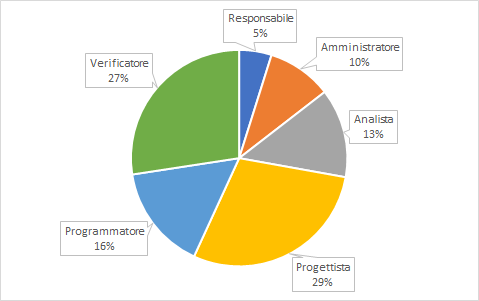
\includegraphics[width=0.7\textwidth]{./res/img/progettazioneArchitetturale_pe.png}
			\caption{Prospetto economico del quattordicesimo incremento}
		\end{figure}
\subsubsection{15$^{\circ}$ Incremento}
		\subsubsubsection{Prospetto orario}
		Durante il quindicesimo incremento la distribuzione oraria preventivata dei ruoli di ogni componente del gruppo sarà la seguente:
		\rowcolors{2}{lightRowColor}{darkRowColor}
		\begin{longtable}{
				>{\centering}p{0.25\textwidth}
				>{\centering}p{0.05\textwidth}
				>{\centering}p{0.05\textwidth}
				>{\centering}p{0.05\textwidth}
				>{\centering}p{0.05\textwidth}
				>{\centering}p{0.05\textwidth}
				>{\centering}p{0.05\textwidth}
				>{\centering\arraybackslash}p{0.15\textwidth} }
			
			\coloredTableHead
			\textbf{\color{white}Nome} &
			\textbf{\color{white}Rp} &
			\textbf{\color{white}As} &
			\textbf{\color{white}An} &
			\textbf{\color{white}Pt} &
			\textbf{\color{white}Pr} &
			\textbf{\color{white}Vf} &
			\textbf{\color{white}Totale}
			\tabularnewline
			\endhead
			
			% Contenuto della tabella
			%    Rp & As & An & Pt & Pr & Vf & Totale \\
			\VB & 1 & -  & - & - & - & - & 1 \\
			\LB & - & -  & - & - & - & - & 0 \\
			\NF & - & -  & - & - & - & - & 0 \\
			\EG & - & -  & - & - & - & - & 0 \\
			\FJ & - & 4  & - & - & - & - & 4 \\
			\MP & 2 & -  & - & - & - & - & 2 \\
			\AS & - & -  & - & - & 1 & 2 & 3 \\
			\AZ & - & -  & - & 2 & - & - & 2 \\
			\textbf{Ore totali per ruolo} & 3 & 4 & 0 & 2 & 1 & 2 & 12 \\
			
			\rowcolor{white}\caption {Suddivisione oraria del quindicesimo incremento} \\
			
		\end{longtable}
		
		% Grafico
		\begin{figure}[H]
			\centering
			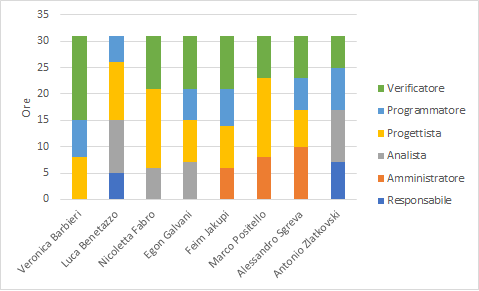
\includegraphics[width=0.7\textwidth]{./res/img/progettazioneArchitetturale_po.png}
			\caption{Suddivisione oraria del quindicesimo incremento}
		\end{figure}
	
		\subsubsubsection{Prospetto economico}
		In base al prospetto orario, quello economico sarà il seguente: 
		\rowcolors{2}{lightRowColor}{darkRowColor}
		\begin{longtable}{
				>{\centering}p{0.25\textwidth}
				>{\centering}p{0.05\textwidth}
				>{\centering\arraybackslash}p{0.15\textwidth} }
			
			\coloredTableHead
			\textbf{\color{white}Ruolo} &
			\textbf{\color{white}Ore} &
			\textbf{\color{white}Costo in \euro{}}
			\tabularnewline
			\endhead
			
			% Contenuto della tabella
			% Ruolo & Ore & Costo \\
			Responsabile    & 3  & 90,00 \\
			Amministratore  & 4  & 80,00 \\
			Analista        & 0  & 0,00 \\
			Progettista     & 2  & 44,00 \\
			Programmatore   & 1  & 15,00 \\
			Verificatore    & 2  & 30,00 \\
			\textbf{Totale} & 12 & 259,00 \\
			
			\rowcolor{white}\caption {Prospetto dei costi per il quindicesimo incremento}	\\
			
		\end{longtable}
		
		% Grafico
		Rappresentazione grafica della distribuzione dei ruoli:
		\begin{figure}[H]
			\centering
			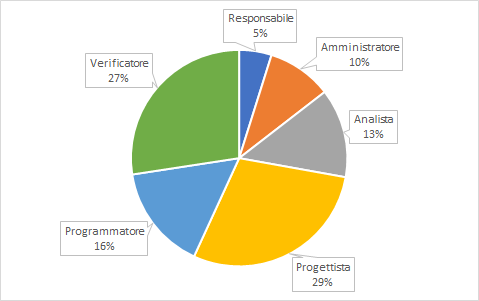
\includegraphics[width=0.7\textwidth]{./res/img/progettazioneArchitetturale_pe.png}
			\caption{Prospetto economico del quindicesimo incremento}
		\end{figure}
\subsubsection{16$^{\circ}$ Incremento}
		\subsubsubsection{Prospetto orario}
		Durante il 16$^{\circ}$ incremento la distribuzione oraria preventivata dei ruoli di ogni componente del gruppo sarà la seguente:
		\rowcolors{2}{lightRowColor}{darkRowColor}
		\begin{longtable}{
				>{\centering}p{0.25\textwidth}
				>{\centering}p{0.05\textwidth}
				>{\centering}p{0.05\textwidth}
				>{\centering}p{0.05\textwidth}
				>{\centering}p{0.05\textwidth}
				>{\centering}p{0.05\textwidth}
				>{\centering}p{0.05\textwidth}
				>{\centering\arraybackslash}p{0.15\textwidth} }
			
			\coloredTableHead
			\textbf{\color{white}Nome} &
			\textbf{\color{white}Rp} &
			\textbf{\color{white}As} &
			\textbf{\color{white}An} &
			\textbf{\color{white}Pt} &
			\textbf{\color{white}Pr} &
			\textbf{\color{white}Vf} &
			\textbf{\color{white}Totale}
			\tabularnewline
			\endhead
			
			% Contenuto della tabella
			%    Rp & As & An & Pt & Pr & Vf & Totale \\
			\VB & - & -  & - & - & - & - & 0 \\
			\LB & - & -  & - & - & - & - & 0 \\
			\NF & - & -  & - & - & - & - & 0 \\
			\EG & - & -  & - & - & - & - & 0 \\
			\FJ & - & -  & - & - & - & - & 0 \\
			\MP & 2 & -  & - & - & - & - & 2 \\
			\AS & - & -  & - & - & 1 & 2 & 3 \\
			\AZ & - & 2  & - & 3 & - & - & 5 \\
			\textbf{Ore totali per ruolo} & 2 & 2 & 0 & 3 & 1 & 2 & 10 \\
			
			\rowcolor{white}\caption {Suddivisione oraria del 16$^{\circ}$ incremento} \\
			
		\end{longtable}
		
		% Grafico
		\begin{figure}[H]
			\centering
			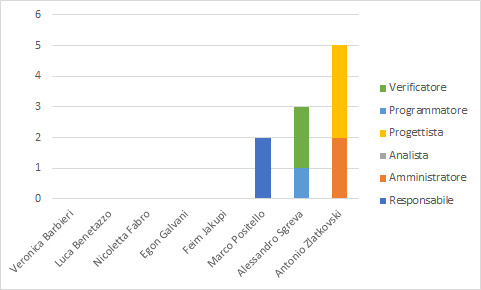
\includegraphics[width=0.7\textwidth]{./res/img/preventivi/inc16_po.png}
			\caption{Suddivisione oraria del 16$^{\circ}$ incremento}
		\end{figure}
	
		\subsubsubsection{Prospetto economico}
		In base al prospetto orario, quello economico sarà il seguente: 
		\rowcolors{2}{lightRowColor}{darkRowColor}
		\begin{longtable}{
				>{\centering}p{0.25\textwidth}
				>{\centering}p{0.05\textwidth}
				>{\centering\arraybackslash}p{0.15\textwidth} }
			
			\coloredTableHead
			\textbf{\color{white}Ruolo} &
			\textbf{\color{white}Ore} &
			\textbf{\color{white}Costo in \euro{}}
			\tabularnewline
			\endhead
			
			% Contenuto della tabella
			% Ruolo & Ore & Costo \\
			Responsabile    & 2  & 60,00 \\
			Amministratore  & 2  & 40,00 \\
			Analista        & 0  & 0,00 \\
			Progettista     & 3  & 66,00 \\
			Programmatore   & 1  & 15,00 \\
			Verificatore    & 2  & 30,00 \\
			\textbf{Totale} & 10 & 211,00 \\
			
			\rowcolor{white}\caption {Prospetto dei costi per il 16$^{\circ}$ incremento}	\\
			
		\end{longtable}
		
		% Grafico
		Rappresentazione grafica della distribuzione dei ruoli:
		\begin{figure}[H]
			\centering
			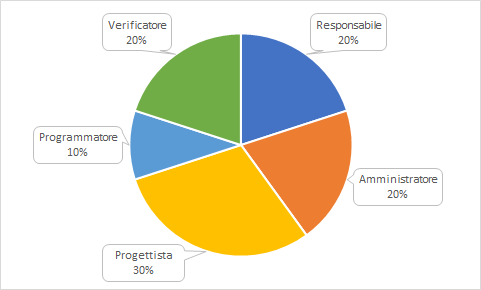
\includegraphics[width=0.7\textwidth]{./res/img/preventivi/inc16_pe.png}
			\caption{Prospetto economico del 16$^{\circ}$ incremento}
		\end{figure}
\subsubsection{Periodo complessivo}

	\subsubsubsection{Consuntivo}
		\begin{longtable}{
			>{\centering}p{0.25\textwidth}
			>{\centering}p{0.08\textwidth}
			>{\centering}p{0.08\textwidth}
			>{\centering}p{0.15\textwidth}
			>{\centering\arraybackslash}p{0.15\textwidth} }
		
		\coloredTableHead
		\textbf{\color{white}Ruolo} &
		\textbf{\color{white}Ore} &
		\textbf{\color{white}Delta ore} &
		\textbf{\color{white}Costo in \euro{}} &
		\textbf{\color{white}Delta costo}
		\tabularnewline
		\endhead
		
		% Contenuto della tabella
		% Ruolo & OreEffettive & DeltaOre & Costo & DeltaCosto \\
		Responsabile    & 23 & +0 &   690,00 & +  0,00 \\
		Amministratore  & 26 & -6 &   520,00 & -  120,00 \\
		Analista        & 3 & +3 &   75,00 & + 75,00 \\
		Progettista     & 94 & +6 & 2068,00 & + 132,00 \\
		Programmatore   & 145 & -8 &   2175,00 &  -120,00 \\
		Verificatore    & 98 & +2 & 1470,00 & + 30,00 \\
		\textbf{Totale Effettivo} & \multicolumn{2}{c}{\textbf{389}} & \multicolumn{2}{c}{\textbf{6998,00}} \\
		\textbf{Delta} & \multicolumn{2}{c}{\textbf{-3}} & \multicolumn{2}{c}{\textbf{-3,00}} \\
		
		\rowcolor{white}\caption{Consuntivo per il periodo di Progettazione di Dettaglio e Codifica}	\\
		
	\end{longtable}
	
	\subsubsubsection{Conclusioni}
	Il bilancio finale è \textbf{positivo}, con un risparmio di \textbf{3,00\euro}. \\ Come riportato nella tabella del consuntivo per il periodo di Progettazione di Dettaglio e Codifica, il numero di ore preventivate per il ruolo di Responsabile si è dimostrato adeguato. \\ Segue un'analisi delle motivazioni per cui gli altri ruoli hanno necessitato di un numero di ore differente da quanto previsto: 
	\begin{itemize}
		\item \textbf{Amministratore}: il numero limitato di modifiche da apportare alle \NdP hanno portato ad un risparmio di ore;
		\item \textbf{Analista}: al contrario di quanto previsto, è stato necessario apportare ulteriori modifiche all'\AdR, questo ha portato alla necessità di alcune ore di lavoro non preventivate;
		\item \textbf{Progettista}: la scarsa conoscenza dei design pattern e l'esito della Product Baseline hanno portato ad un incremento considerevole delle ore di lavoro richieste da tale ruolo;
		\item \textbf{Programmatore}: il riutilizzo del prototipo creato per la \textit{Technology Baseline} e la ripetizione di pattern di comunicazione tra i vari moduli hanno permesso di risparmiare alcune ore di lavoro;
		\item \textbf{Verificatore}: sono state necessarie alcune ore di lavoro non preventivate per verificare tutte le modifiche apportate alla documentazione;
	\end{itemize}
	
	\subsubsubsection{Preventivo a finire}	
	Date le considerazioni precedenti il preventivo complessivo resta invariato. In particolare il risparmio ottenuto in questo periodo risulta essere alquanto ridotto, e per questo non porta ad alcuna ripianificazione. 
	
	

\subsection{Periodo di Validazione e Collaudo}
Vengono riportati di seguito i consuntivi dei 7 incrementi che costituiscono il periodo considerato.

\subsubsection{17$^{\circ}$ Incremento}
		\subsubsubsection{Prospetto orario}
		Durante il 17$^{\circ}$ incremento la distribuzione oraria preventivata dei ruoli di ogni componente del gruppo sarà la seguente:
		\rowcolors{2}{lightRowColor}{darkRowColor}
		\begin{longtable}{
				>{\centering}p{0.25\textwidth}
				>{\centering}p{0.05\textwidth}
				>{\centering}p{0.05\textwidth}
				>{\centering}p{0.05\textwidth}
				>{\centering}p{0.05\textwidth}
				>{\centering}p{0.05\textwidth}
				>{\centering}p{0.05\textwidth}
				>{\centering\arraybackslash}p{0.15\textwidth} }
			
			\coloredTableHead
			\textbf{\color{white}Nome} &
			\textbf{\color{white}Rp} &
			\textbf{\color{white}As} &
			\textbf{\color{white}An} &
			\textbf{\color{white}Pt} &
			\textbf{\color{white}Pr} &
			\textbf{\color{white}Vf} &
			\textbf{\color{white}Totale}
			\tabularnewline
			\endhead
			
			% Contenuto della tabella
			%    Rp & As & An & Pt & Pr & Vf & Totale \\
			\VB & - & -  & - & 3 & - & 2 & 5 \\
			\LB & - & 3  & - & - & - & - & 3 \\
			\NF & 3 & -  & - & - & - & - & 3 \\
			\EG & - & 3  & - & - & - & 2 & 5 \\
			\FJ & 4 & -  & - & - & - & - & 4 \\
			\MP & - & -  & - & - & 3 & - & 3 \\
			\AS & - & -  & - & - & 2 & - & 2 \\
			\AZ & - & -  & - & - & - & 5 & 5 \\
			\textbf{Ore totali per ruolo} & 7 & 6 & 0 & 3 & 5 & 9 & 30 \\
			
			\rowcolor{white}\caption {Suddivisione oraria del 17$^{\circ}$ incremento} \\
			
		\end{longtable}
		
		% Grafico
		\begin{figure}[H]
			\centering
			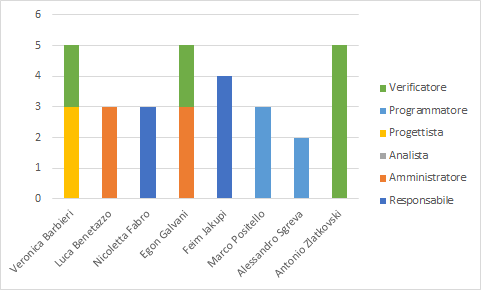
\includegraphics[width=0.7\textwidth]{./res/img/preventivi/inc17_po.png}
			\caption{Suddivisione oraria del 17$^{\circ}$ incremento}
		\end{figure}
	
		\subsubsubsection{Prospetto economico}
		In base al prospetto orario, quello economico sarà il seguente: 
		\rowcolors{2}{lightRowColor}{darkRowColor}
		\begin{longtable}{
				>{\centering}p{0.25\textwidth}
				>{\centering}p{0.05\textwidth}
				>{\centering\arraybackslash}p{0.15\textwidth} }
			
			\coloredTableHead
			\textbf{\color{white}Ruolo} &
			\textbf{\color{white}Ore} &
			\textbf{\color{white}Costo in \euro{}}
			\tabularnewline
			\endhead
			
			% Contenuto della tabella
			% Ruolo & Ore & Costo \\
			Responsabile    & 7  & 210,00 \\
			Amministratore  & 6  & 120,00 \\
			Analista        & 0  & 0,00 \\
			Progettista     & 3  & 66,00 \\
			Programmatore   & 5  & 75,00 \\
			Verificatore    & 9  & 135,00 \\
			\textbf{Totale} & 30 & 606,00 \\
			
			\rowcolor{white}\caption {Prospetto dei costi per il 17$^{\circ}$ incremento}	\\
			
		\end{longtable}
		
		% Grafico
		Rappresentazione grafica della distribuzione dei ruoli:
		\begin{figure}[H]
			\centering
			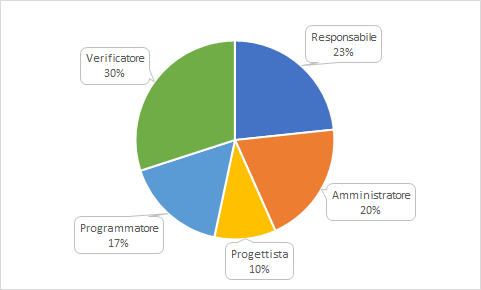
\includegraphics[width=0.7\textwidth]{./res/img/preventivi/inc17_pe.png}
			\caption{Prospetto economico del 17$^{\circ}$ incremento}
		\end{figure}
\subsubsection{18$^{\circ}$ Incremento}

	\subsubsubsection{Consuntivo}
		\begin{longtable}{
				>{\centering}p{0.25\textwidth}
				>{\centering}p{0.08\textwidth}
				>{\centering}p{0.08\textwidth}
				>{\centering}p{0.15\textwidth}
				>{\centering\arraybackslash}p{0.15\textwidth} }

			\coloredTableHead
			\textbf{\color{white}Ruolo} &
			\textbf{\color{white}Ore} &
			\textbf{\color{white}Delta ore} &
			\textbf{\color{white}Costo in \euro{}} &
			\textbf{\color{white}Delta costo}
			\tabularnewline
			\endhead

			% Contenuto della tabella
			% Ruolo & OreEffettive & DeltaOre & Costo & DeltaCosto \\
      Responsabile    & 1  & +0 & 30,00  & +  0,00 \\
      Amministratore  & 1  & +0 & 20,00  & +  0,00 \\
      Analista        & 0  & +0 & 0,00   & +  0,00 \\
      Progettista     & 3  & +0 & 66,00  & +  0,00 \\
      Programmatore   & 10 & +0 & 150,00 & +  0,00 \\
      Verificatore    & 15 & +0 & 225,00 & +  0,00 \\
			\textbf{Totale Effettivo} & \multicolumn{2}{c}{\textbf{30}} & \multicolumn{2}{c}{\textbf{491,00}} \\
			\textbf{Delta} & \multicolumn{2}{c}{\textbf{0}} & \multicolumn{2}{c}{\textbf{+0,00}} \\

			\rowcolor{white}\caption{Consuntivo per il 18$^{\circ}$ Incremento}	\\

		\end{longtable}

	\subsubsubsection{Conclusioni}
	In questo periodo ci siamo dedicati all'implementazione della funzionalità di \texttt{init} (visualizzazione informazioni utili per iniziare ad utilizzare l'applicativo), \texttt{whoami} (visualizzazione dell'indirizzo dell'utente attualmente autenticato nel sistema) e \texttt{search} (ricerca di una funzione). Queste funzionalità richiedono solamente modifiche al modulo \textit{Etherless-cli}, e sono state rispettate il monte ore e le scadenze previste.

	\subsubsubsection{Preventivo a finire rispetto al periodo}
	La pianificazione in questo incremento è stata rispettata e il bilancio risulta essere \textbf{pari}.

	\subsubsubsection{Preventivo a finire complessivo}
	Date le considerazioni precedenti, il preventivo complessivo resta invariato.

\subsubsection{19$^{\circ}$ Incremento}
		
	\subsubsubsection{Consuntivo}
		\begin{longtable}{
				>{\centering}p{0.25\textwidth}
				>{\centering}p{0.08\textwidth}
				>{\centering}p{0.08\textwidth}
				>{\centering}p{0.15\textwidth}
				>{\centering\arraybackslash}p{0.15\textwidth} }
			
			\coloredTableHead
			\textbf{\color{white}Ruolo} &
			\textbf{\color{white}Ore} &
			\textbf{\color{white}Delta ore} &
			\textbf{\color{white}Costo in \euro{}} &
			\textbf{\color{white}Delta costo}
			\tabularnewline
			\endhead
			
			% Contenuto della tabella
			% Ruolo & OreEffettive & DeltaOre & Costo & DeltaCosto \\
			Responsabile    & 1 & +0 &   30,00 & +  0,00 \\
			Amministratore  & 1 & +0 &   20,00 & +  0,00 \\
			Analista        & 0 & +0 &   0,00 & + 0,00 \\
			Progettista     & 2 & +0 & 44,00 & + 0,00 \\
			Programmatore   & 8 & +0 &   120,00 &  +0,00 \\
			Verificatore    & 5 & +0 & 75,00 & + 0,00 \\
			\textbf{Totale Effettivo} & \multicolumn{2}{c}{\textbf{17}} & \multicolumn{2}{c}{\textbf{289,00}} \\
			\textbf{Delta} & \multicolumn{2}{c}{\textbf{0}} & \multicolumn{2}{c}{\textbf{+0,00}} \\
			
			\rowcolor{white}\caption{Consuntivo per il 19$^{\circ}$ Incremento}	\\
			
		\end{longtable}
		
	
	\subsubsubsection{Conclusioni}
	In questo periodo il gruppo si è dedicato principalmente all'implementazione della funzionalità di visualizzazione della cronologia di esecuzione dell'utente. Poichè tale funzionalità richiede delle modifiche unicamente al modulo\ped{\textit{G}} \textit{Etherless-cli} il gruppo è riuscito a rispettare la pianificazione. 
		
	\subsubsubsection{Preventivo a finire rispetto al periodo}
	La pianificazione in questo incremento è stata rispettata e il bilancio risulta essere \textbf{pari}. 
		
	\subsubsubsection{Preventivo a finire complessivo}	
	Date le considerazioni precedenti, il preventivo complessivo resta invariato.
\subsubsection{20$^{\circ}$ Incremento}
		
	\subsubsubsection{Consuntivo}
		\begin{longtable}{
				>{\centering}p{0.25\textwidth}
				>{\centering}p{0.08\textwidth}
				>{\centering}p{0.08\textwidth}
				>{\centering}p{0.15\textwidth}
				>{\centering\arraybackslash}p{0.15\textwidth} }
			
			\coloredTableHead
			\textbf{\color{white}Ruolo} &
			\textbf{\color{white}Ore} &
			\textbf{\color{white}Delta ore} &
			\textbf{\color{white}Costo in \euro{}} &
			\textbf{\color{white}Delta costo}
			\tabularnewline
			\endhead
			
			% Contenuto della tabella
			% Ruolo & OreEffettive & DeltaOre & Costo & DeltaCosto \\
			Responsabile    & 1 & +0 &   30,00 & +  0,00 \\
			Amministratore  & 1 & +0 &   20,00 & +  0,00 \\
			Analista        & 0 & +0 &   0,00 & + 0,00 \\
			Progettista     & 2 & +0 &  44,00 & + 0,00 \\
			Programmatore   & 9 & +4 &   105,00 &  +30,00 \\
			Verificatore    & 5 & +0 & 75,00 & + 0,00 \\
			\textbf{Totale Effettivo} & \multicolumn{2}{c}{\textbf{18}} & \multicolumn{2}{c}{\textbf{274,00}} \\
			\textbf{Delta} & \multicolumn{2}{c}{\textbf{+4}} & \multicolumn{2}{c}{\textbf{+30,00}} \\
			
			\rowcolor{white}\caption{Consuntivo per il 20$^{\circ}$ Incremento}	\\
			
		\end{longtable}
		
	
	\subsubsubsection{Conclusioni}
	In questo periodo il gruppo si è dedicato principalmente all'implementazione della funzionalità di modifica di una funzione. Pur seguendo un pattern di comunicazione tra moduli già utilizzato dal gruppo, l'implementazione della funzionalità ha richiesto più tempo di quanto preventivato. 
	
	\subsubsubsection{Preventivo a finire rispetto al periodo}
	Sono state utilizzare 4 ore di lavoro non preventivate da parte dei Programmatori; questo ha portato ad un bilancio \textbf{negativo}, con una spesa in eccesso di \textbf{30,00\euro}. 
		
	\subsubsubsection{Preventivo a finire complessivo}	
	Non essendo tale spesa eccessiva e avendo ottenuto un risparmio nei periodi precedenti, il preventivo complessivo resta invariato.
\subsubsection{21$^{\circ}$ Incremento}
		\subsubsubsection{Prospetto orario}
		Durante il 21$^{\circ}$ incremento la distribuzione oraria preventivata dei ruoli di ogni componente del gruppo sarà la seguente:
		\rowcolors{2}{lightRowColor}{darkRowColor}
		\begin{longtable}{
				>{\centering}p{0.25\textwidth}
				>{\centering}p{0.05\textwidth}
				>{\centering}p{0.05\textwidth}
				>{\centering}p{0.05\textwidth}
				>{\centering}p{0.05\textwidth}
				>{\centering}p{0.05\textwidth}
				>{\centering}p{0.05\textwidth}
				>{\centering\arraybackslash}p{0.15\textwidth} }
			
			\coloredTableHead
			\textbf{\color{white}Nome} &
			\textbf{\color{white}Rp} &
			\textbf{\color{white}As} &
			\textbf{\color{white}An} &
			\textbf{\color{white}Pt} &
			\textbf{\color{white}Pr} &
			\textbf{\color{white}Vf} &
			\textbf{\color{white}Totale}
			\tabularnewline
			\endhead
			
			% Contenuto della tabella
			%    Rp & As & An & Pt & Pr & Vf & Totale \\
			\VB & - & -  & - & - & 2 & 5 & 7 \\
			\LB & - & -  & - & - & 4 & - & 4 \\
			\NF & - & -  & - & - & 3 & 5 & 8 \\
			\EG & - & -  & - & 2 & - & 1 & 3 \\
			\FJ & - & 3  & - & - & 2 & - & 5 \\
			\MP & 3 & -  & - & - & 1 & 5 & 9 \\
			\AS & - & -  & - & - & 1 & 6 & 7 \\
			\AZ & - & -  & - & 2 & 3 & - & 5 \\
			\textbf{Ore totali per ruolo} & 3 & 3 & 0 & 4 & 16 & 22 & 48 \\
			
			\rowcolor{white}\caption {Suddivisione oraria del 21$^{\circ}$ incremento} \\
			
		\end{longtable}
		
		% Grafico
		\begin{figure}[H]
			\centering
			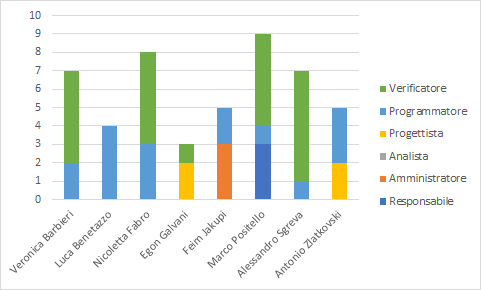
\includegraphics[width=0.7\textwidth]{./res/img/preventivi/inc21_po.png}
			\caption{Suddivisione oraria del 21$^{\circ}$ incremento}
		\end{figure}
	
		\subsubsubsection{Prospetto economico}
		In base al prospetto orario, quello economico sarà il seguente: 
		\rowcolors{2}{lightRowColor}{darkRowColor}
		\begin{longtable}{
				>{\centering}p{0.25\textwidth}
				>{\centering}p{0.05\textwidth}
				>{\centering\arraybackslash}p{0.15\textwidth} }
			
			\coloredTableHead
			\textbf{\color{white}Ruolo} &
			\textbf{\color{white}Ore} &
			\textbf{\color{white}Costo in \euro{}}
			\tabularnewline
			\endhead
			
			% Contenuto della tabella
			% Ruolo & Ore & Costo \\
			Responsabile    & 3  & 90,00 \\
			Amministratore  & 3  & 60,00 \\
			Analista        & 0  & 0,00 \\
			Progettista     & 4  & 88,00 \\
			Programmatore   & 16  & 240,00 \\
			Verificatore    & 22  & 330,00 \\
			\textbf{Totale} & 48 & 808,00 \\
			
			\rowcolor{white}\caption {Prospetto dei costi per il 21$^{\circ}$ incremento}	\\
			
		\end{longtable}
		
		% Grafico
		Rappresentazione grafica della distribuzione dei ruoli:
		\begin{figure}[H]
			\centering
			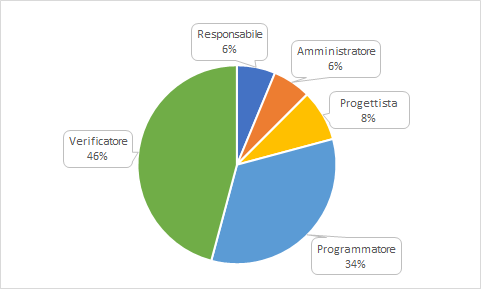
\includegraphics[width=0.7\textwidth]{./res/img/preventivi/inc21_pe.png}
			\caption{Prospetto economico del 21$^{\circ}$ incremento}
		\end{figure}
\subsubsection{22$^{\circ}$ Incremento}
		\subsubsubsection{Prospetto orario}
		Durante il 22$^{\circ}$ Incremento la distribuzione oraria preventivata dei ruoli di ogni componente del gruppo sarà la seguente:
		\rowcolors{2}{lightRowColor}{darkRowColor}
		\begin{longtable}{
				>{\centering}p{0.25\textwidth}
				>{\centering}p{0.05\textwidth}
				>{\centering}p{0.05\textwidth}
				>{\centering}p{0.05\textwidth}
				>{\centering}p{0.05\textwidth}
				>{\centering}p{0.05\textwidth}
				>{\centering}p{0.05\textwidth}
				>{\centering\arraybackslash}p{0.15\textwidth} }
			
			\coloredTableHead
			\textbf{\color{white}Nome} &
			\textbf{\color{white}Rp} &
			\textbf{\color{white}As} &
			\textbf{\color{white}An} &
			\textbf{\color{white}Pt} &
			\textbf{\color{white}Pr} &
			\textbf{\color{white}Vf} &
			\textbf{\color{white}Totale}
			\tabularnewline
			\endhead
			
			% Contenuto della tabella
			%    Rp & As & An & Pt & Pr & Vf & Totale \\
			\VB & - & -  & - & - & - & 2 & 2 \\
			\LB & - & -  & - & - & 2 & 3 & 5 \\
			\NF & - & -  & - & - & - & 5 & 5 \\
			\EG & - & 2  & - & 1 & - & 3 & 6 \\
			\FJ & - & 2  & - & - & - & - & 2 \\
			\MP & 2 & -  & - & - & - & - & 2 \\
			\AS & 5 & -  & - & - & - & - & 5 \\
			\AZ & - & -  & - & 2 & - & 1 & 3 \\
			\textbf{Ore totali per ruolo} & 7 & 4 & 0 & 3 & 2 & 14 & 30 \\
			
			\rowcolor{white}\caption {Suddivisione oraria del 22$^{\circ}$ Incremento} \\
			
		\end{longtable}
		
		% Grafico
		\begin{figure}[H]
			\centering
			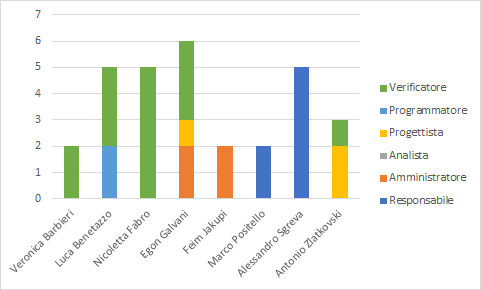
\includegraphics[width=0.7\textwidth]{./res/img/preventivi/inc22_po.png}
			\caption{Suddivisione oraria del 22$^{\circ}$ Incremento}
		\end{figure}
	
		\subsubsubsection{Prospetto economico}
		In base al prospetto orario, quello economico sarà il seguente: 
		\rowcolors{2}{lightRowColor}{darkRowColor}
		\begin{longtable}{
				>{\centering}p{0.25\textwidth}
				>{\centering}p{0.05\textwidth}
				>{\centering\arraybackslash}p{0.15\textwidth} }
			
			\coloredTableHead
			\textbf{\color{white}Ruolo} &
			\textbf{\color{white}Ore} &
			\textbf{\color{white}Costo in \euro{}}
			\tabularnewline
			\endhead
			
			% Contenuto della tabella
			% Ruolo & Ore & Costo \\
			Responsabile    & 7  & 210,00 \\
			Amministratore  & 4  & 80,00 \\
			Analista        & 0  & 0,00 \\
			Progettista     & 3  & 66,00 \\
			Programmatore   & 2  & 30,00 \\
			Verificatore    & 14  & 210,00 \\
			\textbf{Totale} & 30 & 596,00 \\
			
			\rowcolor{white}\caption {Prospetto dei costi per il 22$^{\circ}$ Incremento}	\\
			
		\end{longtable}
		
		% Grafico
		Rappresentazione grafica della distribuzione dei ruoli:
		\begin{figure}[H]
			\centering
			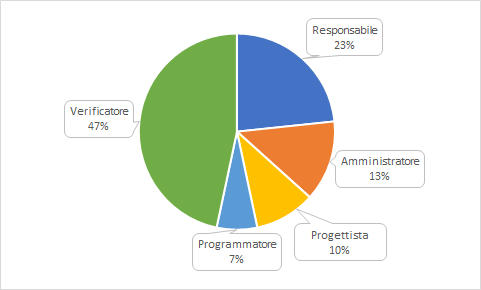
\includegraphics[width=0.7\textwidth]{./res/img/preventivi/inc22_pe.png}
			\caption{Prospetto economico del 22$^{\circ}$ Incremento}
		\end{figure}
\subsubsection{23$^{\circ}$ Incremento}
		\subsubsubsection{Prospetto orario}
		Durante il ventitreesimo incremento la distribuzione oraria preventivata dei ruoli di ogni componente del gruppo sarà la seguente:
		\rowcolors{2}{lightRowColor}{darkRowColor}
		\begin{longtable}{
				>{\centering}p{0.25\textwidth}
				>{\centering}p{0.05\textwidth}
				>{\centering}p{0.05\textwidth}
				>{\centering}p{0.05\textwidth}
				>{\centering}p{0.05\textwidth}
				>{\centering}p{0.05\textwidth}
				>{\centering}p{0.05\textwidth}
				>{\centering\arraybackslash}p{0.15\textwidth} }
			
			\coloredTableHead
			\textbf{\color{white}Nome} &
			\textbf{\color{white}Rp} &
			\textbf{\color{white}As} &
			\textbf{\color{white}An} &
			\textbf{\color{white}Pt} &
			\textbf{\color{white}Pr} &
			\textbf{\color{white}Vf} &
			\textbf{\color{white}Totale}
			\tabularnewline
			\endhead
			
			% Contenuto della tabella
			%    Rp & As & An & Pt & Pr & Vf & Totale \\
			\VB & - & -  & - & - & - & - & 0 \\
			\LB & - & -  & - & - & - & - & 0 \\
			\NF & 1 & -  & - & - & - & - & 1 \\
			\EG & - & -  & - & 1 & - & 2 & 3 \\
			\FJ & - & 1  & - & - & 1 & - & 2 \\
			\MP & - & -  & - & - & - & - & 0 \\
			\AS & 1 & -  & - & - & - & - & 1 \\
			\AZ & - & -  & - & - & - & - & 0 \\
			\textbf{Ore totali per ruolo} & 2 & 1 & 0 & 1 & 1 & 2 & 7 \\
			
			\rowcolor{white}\caption {Suddivisione oraria del ventitreesimo incremento} \\
			
		\end{longtable}
		
		% Grafico
		\begin{figure}[h]
			\centering
			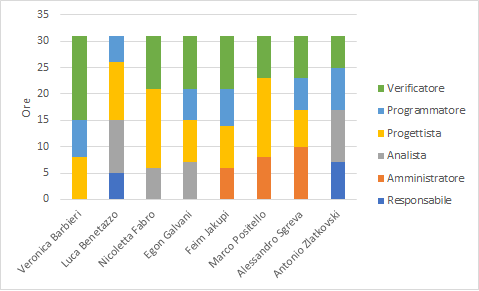
\includegraphics[width=0.7\textwidth]{./res/img/progettazioneArchitetturale_po.png}
			\caption{Suddivisione oraria del ventitreesimo incremento}
		\end{figure}
	
		\subsubsubsection{Prospetto economico}
		In base al prospetto orario, quello economico sarà il seguente: 
		\rowcolors{2}{lightRowColor}{darkRowColor}
		\begin{longtable}{
				>{\centering}p{0.25\textwidth}
				>{\centering}p{0.05\textwidth}
				>{\centering\arraybackslash}p{0.15\textwidth} }
			
			\coloredTableHead
			\textbf{\color{white}Ruolo} &
			\textbf{\color{white}Ore} &
			\textbf{\color{white}Costo in \euro{}}
			\tabularnewline
			\endhead
			
			% Contenuto della tabella
			% Ruolo & Ore & Costo \\
			Responsabile    & 2  & 60,00 \\
			Amministratore  & 1  & 20,00 \\
			Analista        & 0  & 0,00 \\
			Progettista     & 1  & 22,00 \\
			Programmatore   & 1  & 15,00 \\
			Verificatore    & 2  & 30,00 \\
			\textbf{Totale} & 7 & 147,00 \\
			
			\rowcolor{white}\caption {Prospetto dei costi per il ventitreesimo incremento}	\\
			
		\end{longtable}
		
		% Grafico
		Rappresentazione grafica della distribuzione dei ruoli:
		\begin{figure}[h]
			\centering
			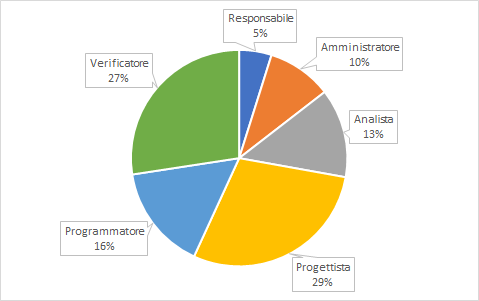
\includegraphics[width=0.7\textwidth]{./res/img/progettazioneArchitetturale_pe.png}
			\caption{Prospetto economico del ventitreesimo incremento}
		\end{figure}
\subsubsection{Periodo complessivo}

	\subsubsubsection{Consuntivo}
		\begin{longtable}{
			>{\centering}p{0.25\textwidth}
			>{\centering}p{0.08\textwidth}
			>{\centering}p{0.08\textwidth}
			>{\centering}p{0.15\textwidth}
			>{\centering\arraybackslash}p{0.15\textwidth} }

		\coloredTableHead
		\textbf{\color{white}Ruolo} &
		\textbf{\color{white}Ore} &
		\textbf{\color{white}Delta ore} &
		\textbf{\color{white}Costo in \euro{}} &
		\textbf{\color{white}Delta costo}
		\tabularnewline
		\endhead

		% Contenuto della tabella
		% Ruolo & OreEffettive & DeltaOre & Costo & DeltaCosto \\
		Responsabile    & 22  & +0 &  660,00  & +  0,00 \\
		Amministratore  & 16  & -1 &  320,00  & - 20,00 \\
		Analista        & 0   & +0 &  0,00    & + 0,00 \\
		Progettista     & 18  & +0 &  396,00  & + 0,00 \\
		Programmatore   & 56  & +9 &  840,00  & + 135,00 \\
		Verificatore    & 71  & -1 &  1065,00 & - 15,00 \\
		\textbf{Totale Effettivo} & \multicolumn{2}{c}{\textbf{183}} & \multicolumn{2}{c}{\textbf{3281,00}} \\
		\textbf{Delta} & \multicolumn{2}{c}{\textbf{+7}} & \multicolumn{2}{c}{\textbf{+100,00}} \\

		\rowcolor{white}\caption{Consuntivo per il periodo di Validazione e Collaudo}	\\

	\end{longtable}

	\subsubsubsection{Conclusioni}
	Il bilancio finale è \textbf{Negativo}, con una spesa in eccesso di \textbf{100,00\euro}. \\ Come riportato nella tabella del consuntivo per il periodo di Validazione e Collaudo, il numero di ore preventivate per il ruolo di Responsabile e Progettista si è dimostrato adeguato. \\ Segue un'analisi delle motivazioni per cui gli altri ruoli hanno necessitato di un numero di ore differente da quanto previsto:
	\begin{itemize}
		\item \textbf{Amministratore}: il numero limitato di modifiche necessarie alle \NdP{} hanno portato ad un risparmio di 1 ora di lavoro;
		\item \textbf{Programmatore}: lo sviluppo di alcuni requisiti desiderabili ha richiesto piú ore del previsto, oltre alla correzione di alcuni errori minori rilevati nel sistema anche in seguito al miglioramento della suite di test rispetto al periodo precedente nel modulo Etherless-cli;
		\item \textbf{Verificatore}: il numero di ore preventivate per questo ruolo si sono rivelate piú che sufficienti allo svolgimento delle attivitá di verifica.
	\end{itemize}

	\subsubsubsection{Preventivo a finire}
	Il bilancio finale del periodo risulta \textbf{Negativo}. Arrivare all'ultima fase del progetto con un bilancio di periodo negativo non é certamente ottimale, tuttavia grazie al risparmio durante i periodi precedenti questo costo in eccesso viene bilanciato e il progetto viene concluso senza eccessi rispetto al preventivo.

